%% Formule de l'operateur : Filtre_spectral_1D
%% Dans ce fichier, les �ventuels accents sont cod�s
%% en ISO-8859-15 (aka latin9)
%% La ligne suivante donne trois exemples 
%% e accent aigu : �, e accent grave : �, e-dans-l'o : �

A chaque pas de temps, le spectre du signal est calcul� par FFT. Ce spectre est multipli� par une gaussienne centr�e sur les plus basses fr�quences. 
La largeur de la gaussienne est fonction du param�tre $W$ qui varie de 0 � 1 (voir figure \ref{fig-filtre-gauss-spectral})
Si $W=0$ il n'y a aucun filtrage, lorsque $W$ tend vers 1 la plage de fr�quences filtr�es
est plus large.  

Les valeurs du profil pour lesquelles $z < z_{min}$ sont interpol�es lin�airement entre 0 et la valeur $X(z_{min})$ ($Type\_{extrap}='lin'$), ou mis � la valeur $X(z_{min})$ ($Type\_{extrap}='cst'$).

\begin{center}

\begin{figure}[htbp]
\centering
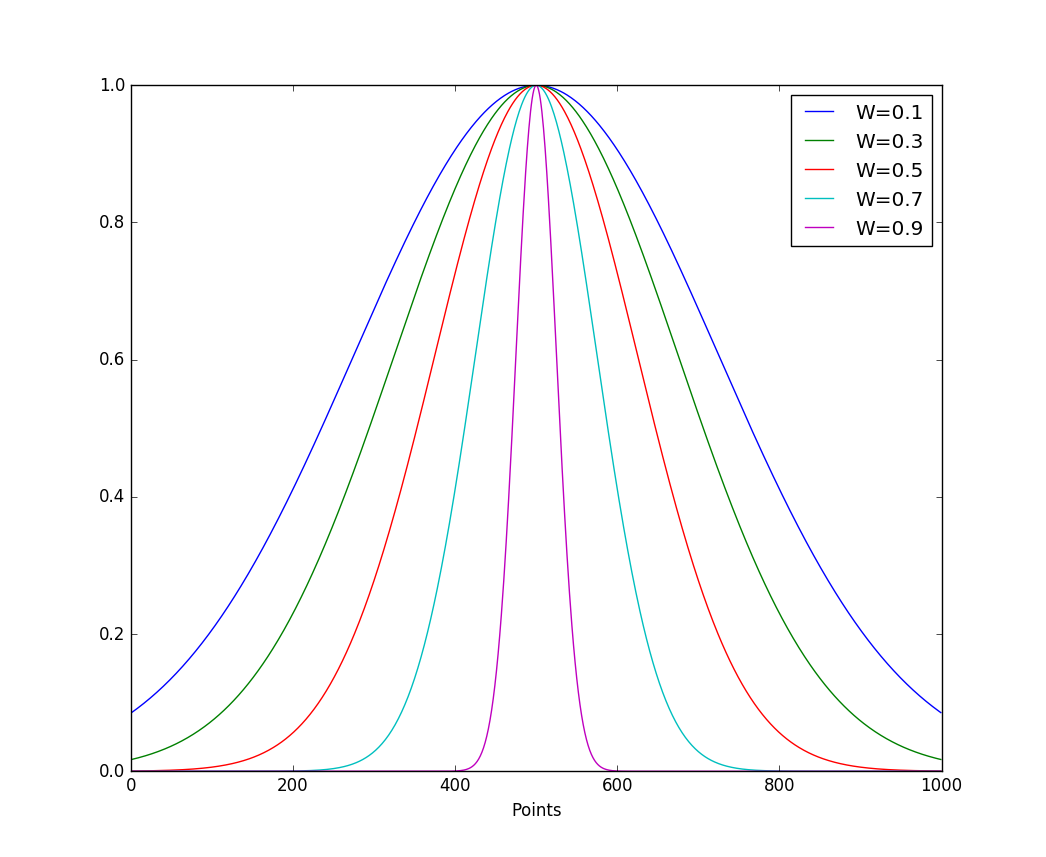
\includegraphics[scale=0.3]{./images/gaussiennes_filtre_spectral_1D.png}
\caption{Gaussienne appliqu�e � la FFT du signal en fonction du param�tre W}
\label{fig-filtre-gauss-spectral}
\end{figure}

\end{center}